% (fold)
% Template: LaTeX file for ICMC 2010 papers, with hyper-references
%
% derived from the DAFx-06 templates
% derived from the ICMC 2009 templates by Steve Beck
%
% 1) Please compile using latex or pdflatex.
% 2) Please use figures in vectorial format (.pdf); .png or .jpg are working otherwise 
% 3) Please use the "papertitle" and "pdfauthor" commands defined below

%------------------------------------------------------------------------------------------
\documentclass[twoside,10pt]{article}
\usepackage{icmc2010,amssymb,amsmath}
\usepackage{bibspacing} 
%\setcounter{page}{1}

\usepackage{listings}						% required for source code listings
\lstset{language=c++}
\lstset{basicstyle=\small\ttfamily}
\lstset{commentstyle=\color{commentcolor}}
\lstset{tabsize=2}
\lstset{gobble=2}							% eat the first tab in block listings
\lstset{aboveskip=\bigskipamount}			% amount of space above a block listing
\lstset{belowskip=\bigskipamount}			% ...

\usepackage{mathptmx} 

%____________________________________________________________
%  !  !  !  !  !  !  !  !  !  !  !  ! user defined variables  !  !  !  !  !  !  !  !  !  !  !  !  !  !
%==== set the title ====
\def\papertitle{A Flexible and Dynamic C++ Framework and Library for Digital Audio Signal Processing}
%\def\papertitle{}	%-- should be empty for the submission anyway!

%==== 1st submission: author name and affiliation are empty for anonymous submission ====
\def\paperauthorA{} 
\affiliation{}{}


%==== final submission: author name and affiliation ====
%---- uncomment 1 to 4 lines, for 1 to 4 authors
\def\paperauthorA{First Author}
\def\paperauthorB{Second Author}
\def\paperauthorC{Third Author}
\def\paperauthorD{Fourth Author}

%%---- set correspnding affiliation data for...
%%-- 1 author
%\affiliation{\paperauthorA}
%  {School\\ Department, City, Country \\ {\tt \href{mailto:email@domain.icmc}{email@domain.icmc}}}

%%-- 2 authors with same affiliation
%\affiliation{\paperauthorA, \paperauthorB}
%  {School\\ Department, City, Country \\ {\tt \href{mailto:email@domain.icmc}{email@domain.icmc}}}

%-- 2 authors with different affiliations
%\twoaffiliations{\paperauthorA}{School\\ Department}
%  {\paperauthorB}{Company\\ Address}

%%-- 3 authors with different affiliations
%\threeaffiliations{\paperauthorA}{School A\\ Department X}
%  {\paperauthorB}{Company\\ Address}
%  {\paperauthorC}{School B\\ Department Y}

%%-- 4 authors with different affiliations
%\fouraffiliations{\paperauthorA}{School A\\ Department X}
%  {\paperauthorB}{Company\\ Address}
%  {\paperauthorC}{School B\\ Department Y}
%  {\paperauthorD}{School C\\ Department Z}

%  ^  ^  ^  ^  ^  ^  ^  ^  ^  ^ user defined variables  ^  ^  ^  ^  ^  ^  ^  ^  ^  ^  ^  ^ 
%------------------------------------------------------------------------------------------

%%-- if using .ps or .eps figure files, they will be converted on the fly
%%-- RMK: for faster LaTeX runs, use it only once after adding new \includegraphics[]{} cmds
%\usepackage{epstopdf}	 

%---- the hyperref package must be last to properly work
\usepackage[pdftex,
       pdftitle={\papertitle},
	pdfauthor={\paperauthorA},
	colorlinks=false,bookmarksnumbered,pdfstartview=XYZ]{hyperref}
%\pdfcompresslevel=9
\usepackage[pdftex]{graphicx}	% for compatible graphics with hyperref
\usepackage[figure,table]{hypcap}	% corrects the hyper-anchor of figures/tables

% Stuff added by [tap]
\usepackage{hyperref}
\usepackage{url}
\usepackage{amsmath}
\usepackage{color}
\definecolor{black}{rgb}{0,0,0}
\hypersetup{colorlinks
,linkcolor=black
,filecolor=black
,urlcolor=black
,citecolor=black}
%reduces the space between the items in the itemize-environment 
\newenvironment{packed_item}{
\begin{itemize}
  \setlength{\itemsep}{1pt}
  \setlength{\parskip}{0pt}
  \setlength{\parsep}{0pt}
}{\end{itemize}}



\title{\papertitle}
% (end)

%------------------------------------------------------------------------------------------
\begin{document}
\sloppy
\DeclareGraphicsExtensions{.png,.jpg,.pdf} % used graphic file format for pdflatex
    
\maketitle

%%%%%%%%%%%%%%%%%%%%%%%%%%%%%%%%%%%%%%%%%%%%%%%%%%%%%%%%%%%%%%%%%%%%%%%%%%%%%%%%%%%%%%%%%%%

\begin{abstract}

This paper presents an object-oriented, reflective, application programming interface for C++, with an emphasis on real-time signal processing. 
The Jamoma Foundation and DSP Library provide a flexible framework and runtime environment, as well as an expanding collection of unit generators for synthesis, processing, and analysis.  It makes use of polymorphic typing, dynamic binding, and introspection to create a cross-platform environment pulling ideas from languages such as Smalltalk and Objective-C while remaining within the bounds of the portable and cross-platform C++ context. 
This library has been used in both open source and commercial software projects over the past several years.

\end{abstract}


%%%%%%%%%%%%%%%%%%%%%%%%%%%%%%%%%%%%%%%%%%%%%%%%%%%%%%%%%%%%%%%%%%%%%%%%%%%%%%%%%%%%%%%%%%%

\section{Introduction} % (fold)
\label{sec:introduction}

``The SMC Roadmap identifies two broad research challenges: (1) To design better sound objects and environments and (2) To understand, model, and improve human interaction with sound and music.'' \cite{serra:2007}  The Jamoma Foundation and DSP Library directly addresses the first task as a means by which to address the second task.  Before discussing the approach and relative merits taken in the Jamoma project, we will first lay out some definitions and quickly review similar projects.


\subsection{Terminology} % (fold)

For the course of the paper, the usage of various computer science jargon and terminology needs to be defined.  In \emph{object-oriented programming} functionality related to a set of data is treated as a unit.  These units, or objects, are created and then often passed using a reference or pointer to the memory in which the object's contents are stored.  These objects comprise \emph{methods} (functions) and \emph{attributes} (properties or data which represent part of an object's state).

\textbf{Polymorphism} is a means by which a programming language generalizes different types of functions or data using a common \emph{API}, or Application Programming Interface.  An example of a polymorphic data-type of the variety in which we are interested is a `var' in the Javascript language\cite{Flanagan:2002}.  That is to say a data type which may be any data type internally (including an object or array), the details of which are not necessary in order to use or pass the data type amongst functions.

\textbf{Introspection} refers to the ability to determine the characteristics of an object at runtime.  This means that when handed a pointer in C++, we can take the pointer and query for an object's name, its type or \emph{class}, the messages that it understands, the attributes it possesses, etc.  By extension, \textbf{reflection} refers to the ability to then modify the behavior of an object at runtime\cite{Malenfant:1996}.  In practical terms this means adding messages, changing attributes, and extending existing instances of objects as the software is executing and without stopping the software to re-compile the code.

Introspection and reflection are often implemented by making use of a \textbf{dynamic binding model}.  Programming languages including C++ and Java link function and method calls when a program is compiled, known as static binding.  A dynamically bound model does not link these functions at compile-time, but instead waits until runtime to resolve the address of a method being called.  When a dynamic binding model is in use, calling methods is referred to as `sending messages' to objects. Dynamic binding is the hallmark of languages like Smalltalk \cite{Krasner:1988}, Objective-C \cite{Cox:1986}, or Ruby.

Throughout the literature exists a confusing gaggle of terminology for classifying systems of objects.  These include \emph{framework}, \emph{library}, \emph{environment}, and \emph{toolkit}.  For the purposes of this paper, these will be defined as follows.  
A \textbf{unit generator} is a class or object that implements a well-defined DSP task such as generating, analyzing, or processing audio data.
A \textbf{library} is a collection of pre-built and ready-to-use unit generators.
A \textbf{toolkit} is a collection of functions, utilities and helpers, possibly with an API, for creating unit generators.
A \textbf{framework} is an architectural structure that underlies a system of unit generators.
A \textbf{runtime} is a daemon or framework operating in real-time when a framework, toolkit, or unit generator is in use. A runtime's role is typically for dispatching messages, balancing processor loads, or otherwise running the background machinery such as in the Objective-C or Java runtime environments.
An \textbf{environment} is a full-fledged system intended for use by an end-user.  Examples include Max, SuperCollider, ChucK, DAW applications, and CSound.
%(end)


\subsection{Requirements} \label{sec:Requirements}% (fold)

The authors are involved in a number of divergent and parallel efforts requiring both a framework for creating unit generators and a library of ready-to-go unit generators.  These efforts include both open-source and closed-source commercial applications targeting multiple platforms and environments.  To meet the manifold demands of these endeavors the following list of requirements must be met regarding how said framework must perform and behave.

% TODO: Nils, Trond and both agreed that we needed bullets here.  However, maybe there is a way to justify them further to the left?

\begin{packed_item}%\begin{itemize}
  \item \textbf{Licensing} allows for both open source and commercial use
	\item \textbf{Cross-platform} compliant (Mac, Windows, Linux, Embedded Devices, Mobile Platforms)	
	\item \textbf{64-bit} audio bit-depth
	\item \textbf{Multichannel audio support}
	\item \textbf{Reasonably efficient},i.e. frame-based audio processing
	\item \textbf{User-extensible} (adding functionalities without recompiling core frameworks)
	\item \textbf{Dynamically reconfigurable} classes at runtime (dynamic-binding)
	\item \textbf{Adaptable} process method to varying input (frame sizes, channel configurations, etc.) on-the-fly
	\item \textbf{Effortless use} of classes in different environments (Max/MSP, VST, AudioUnit, ChucK, Pd)
%	\item be as thread-agnostic as possible (don't manage it, but take care of requisite protection, adaptable to various architectures)
%	\item MVC-friendly (reconfigurable)
\end{packed_item}%\end{itemize}

% NOTE: Terms not defined: reconfigure classes, object decoration, process routine switching, frame-based audio processing, thread-agnostic, requisite protection,  MVC [tl]

\noindent Having met these technical requirements, the authors also deem an additional set of process requirements to be important.  These requirements are in adhering to contemporary philosophies for good coding practice, 
which facilitates the readability, debugging, maintenance and distribution of code. 
%ensuring that it is pleasant to work with the code, to maintain it, to test it, and to distribute it.

\begin{packed_item}%\begin{itemize}
	\item expressive syntax, idioms, and conventions
	\item adhere to the DRY (Don't Repeat Yourself) principle, which states that ``Every piece of knowledge must have a single, unambiguous, authoritative representation within a system''\cite{Hunt:1999}
%	\item clear code % what do we mean by this?
	\item convention over configuration\cite{web1}
	\item tag-based searching for class categorization and object instantiation
	\item integrated unit testing and benchmarking\cite{web2}
\end{packed_item}%\end{itemize}

% One list for efficiency to the computer
% One list for efficiency for the development process / programmers's workflow : Ruby : set out top make a program that would "make programmers happy"; "Ruby is simple in appearance, but is very complex inside, just like our human body" - Yukihiro “matz” Matsumoto

% (end)
% (end)


%%%%%%%%%%%%%%%%%%%%%%%%%%%%%%%%%%%%%%%%%%%%%%%%%%%%%%%%%%%%%%%%%%%%%%%%%%%%%%%%%%%%%%%%%%%

\section{Prior Art} % (fold)
\label{sec:prior_art}

A myriad of existing libraries, toolkits, frameworks, and environments are available for digital signal processing.  To justify the effort of creating a new framework the merits of the extant members in this field should be considered, particularly with regard to our previously stated requirements.

% TODO: be clear that we are eliminating existing toolkits in order to justify our creation of a new one?

\subsection{Choice of Language} % (fold)

An immediate winnowing of the field of contenders can be accomplished by discussing the choice of programming language.  There are popular and well structured DSP libraries for Java \cite{Guillemard:2005, Burk:1998} and Objective-C \cite{Jaffe:1989,Jaffe:1991}, for example, but these languages also carry restrictions and baggage.  Java is not installed on Windows systems by default and is not available in the context of many embedded devices.  Objective-C is available on Windows only through the clumsy and inadequate GnuStep project\footnote{For example, one cannot natively compile using Microsoft's MSVC compiler.} \cite{web3} and also is not available in the context of many embedded or mobile devices
%\footnote{The authors also look upon Apple's corporate control of the Objective-C language and runtime with some degree of skepticism, as compared to the open consortium that is mediating the C++ language's evolution}.  
Interpreted languages such as Ruby and Python are quite powerful, but do not provide the required speed for real-time DSP performance in embedded environments and can also create portability problems in some cases. 
%TODO: is there any recent comparison of DSP speed between Java, Python and C ? [NP}  

Another class of languages are domain-specific languages for audio signal processing.  These include SuperCollider\cite{McCartney:1996}, ChucK\cite{wang:2008}, and CSound.  For our purposes we will also consider the Max family (including MSP\cite{Zicarelli:1998} and PureData\cite{Puckette:1996}) to be domain-specific-languages
%\footnote{We acknowledge the heated debate as to whether these environments actually constitute languages and the dispute regarding whether the use of these environments should be considered programming.}
.  
These domain-specific languages do provide facilities both for creating and using Unit Generators, but often have portability limitations and very frequently have licensing limitations\footnote{For example, ChucK and SuperCollider are licensed as GPL and thus not available for commercial development, while Max/MSP is not available on embedded devices nor in plug-in host environments other than Ableton Live}.  These environments also frequently have a large footprint in that they are very resource demanding, while we desire a light-weight framework.

The C++ language and its compilers are ubiquitous across platforms.  Plug-ins and extensions for sundry environments and languages can be compiled using C and C++.  The C++ language is also capable of creating extremely high-performance code optimized for digital signal processing.

% (end)


\subsection{Plug-in APIs} % (fold)

A related subject is the creation of audio plug-ins using existing APIs.  VST, RTAS, LADSSPA/DSSI, and AudioUnits are all APIs for creating UnitGenerators in C/C++.  None of these technologies, however, meet our requirements.  None are actually libraries, though there is a standard set of the non-cross-platform AudioUnit plug-ins provided by Apple.

% (end)


\subsection{Licensing} % (fold)

As stated, the authors require a framework that can be used in both open-source and commercial applications.  This immediately rules out the use of any existing work licensed under the GNU GPL, which stipulates that all works using it are themselves licensed under the GNU GPL.  Among the options this rules out are SndObj \cite{Lazzarini:2001}, CLAM \cite{Amatraian:2008}, and Marsyas \cite{Tzanetakis:2008}.  Additionally, the CSL framework \cite{Pope:2003} requires licensing through the University of California, which is not agreeable to the open use we require.

Due to these licensing restrictions, none of these packages are suitable for our use\footnote{The license for the STK is reasonably liberal.  At the time that the Jamoma DSP library was initially written, however, the license for the STK specified non-commercial use and thus using the STK was not an option for the authors.}.  They do, however, contain many valuable ideas that serve to inform our own work.
% TODO: Will we be touching upon valuable ideas from these libraries later again?

% (end)


\subsection{Dynamic Binding} % (fold)

One of our core concerns is the requirement for dynamically reconfigurable classes at runtime.  For this, dynamic binding is of critical importance.  Dynamic binding is implemented to some degree in many of the aforementioned environments including Marsyas, Max/MSP, and the NeXT SoundKit for Objective-C.  However, due to our cross-platform and liberal licensing requirements they are not options.  Of the remaining DSP libraries and toolkits, the STK\cite{Cook:1999}, CMix \cite{Lansky:1990}, and TANGA \cite{Reiter:2007} are all statically-bound.  

%NOTE: IMHO the second last sentence could be left out, as we have dismissed all the aforementioned libraries already, including Marsyas, Max/MSP and NeXT SoundKit [TL] -- I disagree, we need to make the point that they have dynamic-binding so that we aren't operating in a void for this issue [tap]

An interesting middle-of-the-road option is Kronos.  In fact, the problem domain of the Kronos system is the same as our problem domain: `` the musician may want to change the program during its execution. This was possible in the analog music studio, where swapping out patch cords often resulted in immediate gratification. In the digital world programs often have to be aborted, edited, re-compiled, linked and launched. The all-important musical hacking suffers from such a heavy compilation cycle, making a traditional programming language less desirable for real time artistic expression.'' \cite{Norilo:2009}

Dynamically-bound frameworks and runtimes, such as PureData, Objective-C, or Marsyas, solve this problem by precompiling the unit generators and then directing messages to these objects at runtime.  Kronos takes an alternative approach where the graph of objects, indeed the unit generators themselves, are not precompiled at all but rather compiled `Just in Time' from a custom meta-language. This results in better performance from the code, while still maintaining much of the flexibility offered by a dynamically-bound runtime.  The performance results are compelling.  Unfortunately a just-in-time compilation still requires compilation every time you change the interconnections between objects, and the resulting domain-specific language may be limited to only the domain for which it is written.

One interesting cross-platform, dynamically-bound, and liberally licensed architecture is ZenGarden\cite{web4}.  One feature of ZenGarden is the use of PureDatas an authoring environment to define a graph of ZenGarden's own unit generators, as was done for the popular RjDj iPhone app \cite{web5}.  Unfortunately, at the time of this writing, ZenGarden does not pass our next requirement: 64-bit audio fidelity.

% (end)


\subsection{64-bit Audio} % (fold)

The higher resolution of 64-bit audio improves stability and fidelity in processes that are vulnerable to numerical instability.  This includes IIR filters at extreme settings and signal processing algorithms solving differential equations, as can be the case for physical modeling.  If audio signals are used as wavetable lookup indexes, a 32-bit float signal with a 24-bit signed mantissa is able to address only 6'20" of audio with sample accuracy at 44.1 kHz and no more than 1'26" at 192 kHz. In a 64-bit audio chain this problem will be nonexistent for all practical concerns. The computational overhead required for 64-bit processing is counteracted by the fact that 64-bit processors are becoming increasingly common.

% (end)


\subsection{Conclusion} % (fold)

In the end we found no one framework to possess all of the requirements set forth.  As the de facto standard for audio DSP libraries, the STK comes perilously close as of more recent revisions\cite{Scavone:2005}, and offers a rich and mature array of unit generators.  The STK is statically-bound.  While a problem for the kinds of applications we envision, this does yield potentially faster execution of the code.  We propose an alternative that will not replace the STK, but rather coexist with it as a part of the greater computer music ecology.

% Why in the world do we need another DSP framework?
%
% Section 5 of Amatraian:2008 maybe provide the start of a way to categorize different frameworks.
% I'm not sure if it actually makes sense to distinguish between text and gui interfaces, given that the 
% underlying data-flow basis is exactly the same (as argued in several of the Tzanetakis papers)  
%
% However, I think it is useful to distinguish between Unit Generators (STK, AU, VST), Unit Graphs
% (AUGraph, Multicore, ?), and those that combine both into one (CLAM, Max/MSP, Marsyas)
% [tap]

% (end)

% (end)



%%%%%%%%%%%%%%%%%%%%%%%%%%%%%%%%%%%%%%%%%%%%%%%%%%%%%%%%%%%%%%%%%%%%%%%%%%%%%%%%%%%%%%%%%%%

\section{Platform Architecture} % (fold)
%\section{The Jamoma Platform}
%alternative title: The Jamoma Structure, The Jamoma Universe, the Jamoma Context,  

\subsection{A Layered Framework Structure}

It is common to organize software frameworks into a number of layers from low level system services at the bottom towards high level abstraction at the top.  Frameworks may build upon and extend frameworks below them in the hierarchy, but the lower frameworks have no knowledge of the higher frameworks. Divisions between the frameworks help to establish clarity as to what functionalities belong to which part of the system. 

Examples of such layered architectures are the Open Systems Interconnection network model (OSI) \cite{web6} 
for layered communications and computer network protocol design or the iPhone Software Architecture. A similar layered approach has been proposed by the authors for spatialization systems \cite{Peters:2009}. 

\begin{figure}[htbp]
\centerline{\framebox{
	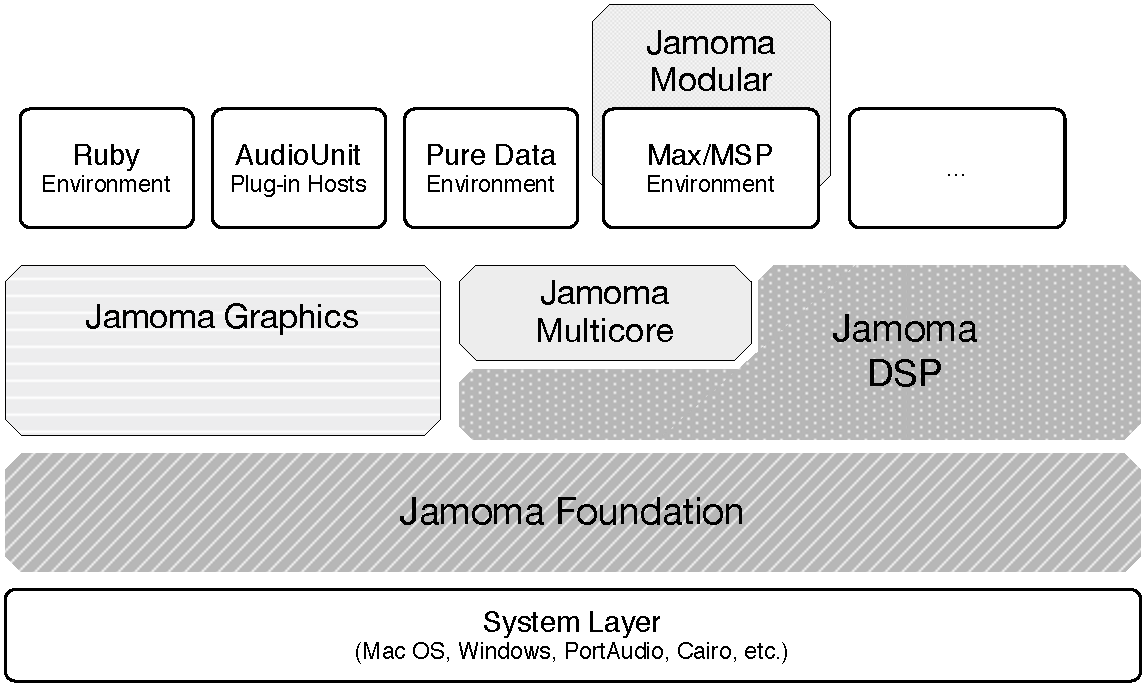
\includegraphics[width=0.9\columnwidth]{layers-alt}}}
\caption{The Jamoma Platform as Layered Architecture.}
\label{fig:layers}
\end{figure}

Jamoma, originally conceived as a modular standard for structuring patchers in Max \cite{Place:2006}, has now evolved into a layered architecture of frameworks providing comprehensive infrastructure for creating computer music systems in general, not just for Max/MSP.  This section presents each of the five frameworks currently comprising the Jamoma Platform: Jamoma Foundation, Jamoma DSP, Jamoma Multicore, Jamoma Graphics and Jamoma Modular (see Figure~\ref{fig:layers}).  We will emphasize the Foundation and DSP layers to illustrate how we meet the requirements outlined in Section \ref{sec:Requirements}.
 
% TODO: be sure to emphasize the  polymorphic typing and dynamic binding throughout this section to tie in to the abstract etc...
  
It is possible to use only a subset of the provided frameworks according to the project's complexity. 
Each framework within the Jamoma Platform shares a common structure.  A shared-library implementing base classes and core functionality exists at the core.  This functionality is then extended and enhanced by creating extensions.  An extension is a plug-in library that is dynamically loaded at runtime.  In this way the system can be expanded without re-compiling core components.


\subsection{Foundation} % (fold)

The Jamoma Foundation \cite{web7} may be seen as analogous to the Objective-C Foundation, which ``Defines the `nuts and bolts' classes for Objective-C programming''\cite{web8}.  The Jamoma Foundation defines base classes, including our primary base class, \texttt{\small{TTObject}}.  Object life-cycle facilities include factories for creating, destroying, and referencing these classes.  A message-passing and attribute system inspired by Smalltalk and Objective-C is implemented to enable dynamically-bound object topologies.  

The Jamoma Foundation classes are informed by many best-practices of software development.  Unit Testing, for example, is integrated directly into the class design.  There is also an emphasis on the use of design patterns \cite{Gamma:1995}.  In particular, all objects possess a built-in observer notification system.  

As much as possible, complexity, `glue code', and the mechanics of writing C++ are hidden from the programmer.  They may be accessed if necessary, however, by relying on a convention-over-configuration paradigm the clarity of the code is dramatically improved.  In the opinions of the authors' this makes the code not only less time consuming to create and maintain, but also more enjoyable.  This aim is also aided by emphasizing DRY principles throughout the Jamoma Platform.

Functionality specific to audio or digital signal processing is not present in this particular framework.  In fact, the Jamoma Foundation can be used as a general framework and runtime as a dynamically-bound API layer on top of C++ for any purpose.  This is evident, for example, in the Jamoma Graphics Library.

\subsubsection{Messages and Attributes} % (fold)

As with other similar runtime systems, the Jamoma Foundation defines a symbol table for efficient message dispatch and lookup.  This symbol table is leveraged in the implementation of messages and attributes.  
A \emph{message} is defined as a method of a class or instance that is then bound to a symbol.  Messages may optionally possess arguments for passing data to and from the object.

An \emph{attribute} is defined as a data member of a class or instance, whose access is bound to symbol.  Typically, the setting or retrieving of the value then uses a built-in accessor method.  If needed, a custom setter or getter method can be defined to override the built-in mechanism.

Additionally, attributes may possess \emph{properties}.  Properties are implemented as attributes of the attribute.  They include the ability define ranges for an attribute, the behavior of an attribute's value when the range is exceeded, etc.  The design of this system is consistent with the authors' previous proposals for more sophisticated control in parametric systems \cite{Place:2008params}.

\subsubsection{Implementation}

To actualize the notion of sending messages to objects, and by extensions setting attributes, the Jamoma Foundation relies upon two primary underpinnings.  First is a polymorphic data-type, \texttt{\small{TTValue}}, that enables us pass data to and from methods regardless of the kind of data actually contained while using a common interface.  %TODO: TTValue does some other cool things...

By using \texttt{\small{TTValue}} to represent any arbitrary data, we are able to abstract the function/method prototype for any message or attribute.  By doing so, we create system by which all communication to and from objects occurs using a singular interface.  Internally the messages and attributes of an object are managed a hash tables (for speed) of pointers.  Changing the contents of the hash table or the values of the pointers at runtime then reconfigures how messages are directed and handled while not requiring any recompiling or relinking of the code.

\texttt{\small{TTObject}} implements and observer pattern by maintaining linked-lists of other objects that wish to be notified of events.  The objects registered as observers are then sent messages from \texttt{\small{TTObject}}.  If the objects respond to the message sent then they can respond appriopriately.  If they do not respond to the message, then they will simply ignore it.  In this case no intervention is required by the user or programmer, and this situation is not considered an error.  In a statically-bound system this situation would likely lead to a compile-failure, thrown exceptions, crashes during operation, or worse.

% (end)
% (end)


\subsection{DSP Layer} % (fold)

The Jamoma DSP Layer \cite{web9} augments the Foundation by extending \texttt{\small{TTObject}} to create a new \texttt{\small{TTAudioObject}} base class.  \texttt{\small{TTAudioObject}} provides the core functionality for processing multichannel, 64-bit, audio samples singly or in blocks while providing basic thread protection.  It also provides attributes and audio processing methods for controlling muting, bypass, sample-rate, etc. which are inherited by subclasses.

In addition to the framework and base-classes, the DSP layer also provides toolkit functionality with convenience functions such as denormals and dc-offset blocking, and a library of classes as extensions implementing a variety of unit generators.  The provided unit generators include basic trigonometry functions, filters (including butterworth), oscillators, noise generators, analysis, effects, etc.  These classes are organized and classified on several different levels.  First, every object is classified using tags when the object is registered with the Foundation at runtime.  The Foundation then manages this registry and its metadata for use by the factory methods for creating instances.  Secondly, the classes are organized into dynamically loaded \emph{extensions} which share common interfaces and functionality.

\subsubsection{Extensions}

User extensions may be created for any of layers built-upon the Jamoma Foundation.  At this time, extensions are almost exclusively for the purpose of creating unit generator classes with Jamoma DSP. An extension may implement zero or more classes, which are registered with the Foundation when the extension is loaded.

The extensions included with Jamoma DSP are organized into groups of classes that share a common interface.  For example, the \emph{FilterLib} implements more than two dozen audio filters including Butterworth and Linkwitz-Riley algorithms for various frequency responses.  All classes in the FilterLib use shared semantics for defining message and attribute names, such as `frequency', and can thus be easily substituted for one another.  Similarly, the \emph{FunctionLib} implements a number of algorithms designed for use gestural mapping scenarios.  

While common attribute and message names are preferred, some unit generators will necessarily provide additional controls when compared to simpler or different classes.  When substituting one class for another, we leverage the dynamically-bound architecture because we can send messages to an object, even if it does not understand them.  In this case the messages are simply ignored.  With introspection features, all classes can be queries to find out what attributes they do possess, what ranges characterize those attributes, etc.  Objects can also be modified at runtime to add handling for messages not envisaged at compile time using reflective techniques, allowing them to be adapted for use in different contexts.

In addition to the FilterLib and FunctionLib, the growing number of extensions for Jamoma DSP include the AnalysisLib, GeneratorLib, MathLib, EffectsLib, and WindowFunctionLib.

%    - common interface for filters - FilterLib
%    - common interface for generators
%    - for functions - also used for mappings and ramps elsewhere
%    - EffectsLib
%    - for windowing functions
%- how to make additional extensions as neeeded or add units to existing extensions
%    - the extensibility of it 
%    - DRY means that this is faster to do, and the code cleaner to read

% (end)


\subsection{Additional Layers} % (fold)

Additional layers have been implemented on top of the Jamoma Foundation, both in series and in parallel with the DSP layer.  

The \textbf{Graphics Layer}\cite{web10}, based on Cairo\cite{web11}, provides both a platform-independent, and a host-independent way to create 2D graphical user interfaces (GUI). It has been used for creating GUIs in Max/MSP and in AudioUnit plug-ins.

The \textbf{Multicore Audio Graph Layer}\cite{web12} combines unit generators from Jamoma DSP into audio processing topologies.  This differs from many of the initiatives reviewed in Section~\ref{sec:prior_art}, as they combined not only a means by which to create unit generators but also a method by which those objects are combined into a graphs.  In the Jamoma Platform we create a clear division between creating and using unit generators versus combining them into a graph.  This allows the unit generators to be combined in any way that seems desirable for a particular context.

The \textbf{Modular Framework}\cite{web13} provides structure for the development and control of modules in the Max/MSP/Jitter environment\cite{Place:2006}.  It builds upon the Foundation, DSP, Graphics, and Multicore frameworks.

% (end)


\subsection{Ruby Language Bindings} % (fold)

As a dynamically-bound API, the Jamoma Foundation is a natural fit for control from the Ruby environment.  Language bindings for Jamoma in Ruby exist via the Jamoma Ruby project\cite{web14}.  This enables use in a wide range of applications including live coding using \emph{irb} \cite{web15} and integration with web applications using \emph{Ruby on Rails} \cite{web16}.

% (end)
% (end)


%%%%%%%%%%%%%%%%%%%%%%%%%%%%%%%%%%%%%%%%%%%%%%%%%%%%%%%%%%%%%%%%%%%%%%%%%%%%%%%%%%%%%%%%%%%

\section{Applications} % (fold)

The technical underpinnings of the Jamoma Foundation and DSP Library lend themselves to a variety of applications.  The API provides a clear interface to both creating and using unit generators in the C++ language or Ruby.  Additional tools and facilities have been fabricated to make Jamoma DSP's unit generators readily available in several popular environments.

% TODO: dynamic-binding - reflective - introspection are leveraged here, we need to make this obvious and explicit

\subsection{Max/MSP}

Given a Jamoma DSP unit generator, this object can be easily compiled for Cycling '74's Max/MSP environment.  The easiest way is to use the Jamoma DSP ``Class Wrapper'', which takes an existing class and creates bindings for the target environment. Following is the complete code listing for an N-channel MSP external that wraps the Jamoma DSP limiter class.

\begin{lstlisting}
  #include "TTClassWrapperMax.h"
  int main(void)
  {
    TTDSPInit();
    return wrapTTClassAsMaxClass(TT("limiter"), 
            "myMaxLimiter~", NULL);
  }
\end{lstlisting}

\noindent In addition to simply wrapping existing classes for MSP, it is possible to use the Jamoma DSP objects in other ways.  One example is the \texttt{\small{jcom.filter$\sim$}} external provided with Jamoma DSP.  
%NOTE: instead of using jcom.filter example, why not using tt.filter example, to show the commercial application [np] -- I think we should mention the items in the distro, and commercial applications are touched upon elsewhere [tap]
This object dynamically loads any of a variety of filter classes from the DSP Library.  The classes are loaded and swapped on-the-fly, without requiring Max's DSP chain to be rebuilt.  The code for the \texttt{\small{jcom.filter$\sim$}} object searches the object registry for available filter classes to present a list of choices for the user.  This list will then be dynamically updated if new filters are added without requiring any code to be compiled or updated.   


\subsection{Plug-ins}

Jamoma DSP provides a number of example projects that include VST and AudioUnit plug-ins.  AudioUnit plug-ins requiring only a generic interface may be created using a class wrapper similar to the one for creating Max/MSP externals.  

The spatial sound rendering technique ViMiC (Virtual Microphone Control) is a virtual multi-microphone recording environment \cite{CMJ08-VIMIC}.  ViMiC is implemented as an AudioUnit plug-in using the Jamoma DSP, Foundation and Graphics frameworks.  The virtual microphones and sound sources can be controlled and manipulated in a custom interface, developed with Jamoma Graphics.  Additional control features are accessible using the generic AudioUnit interface (see Figure \ref{fig:vimic}).


\begin{figure}[htbp]
\centerline{\framebox{
	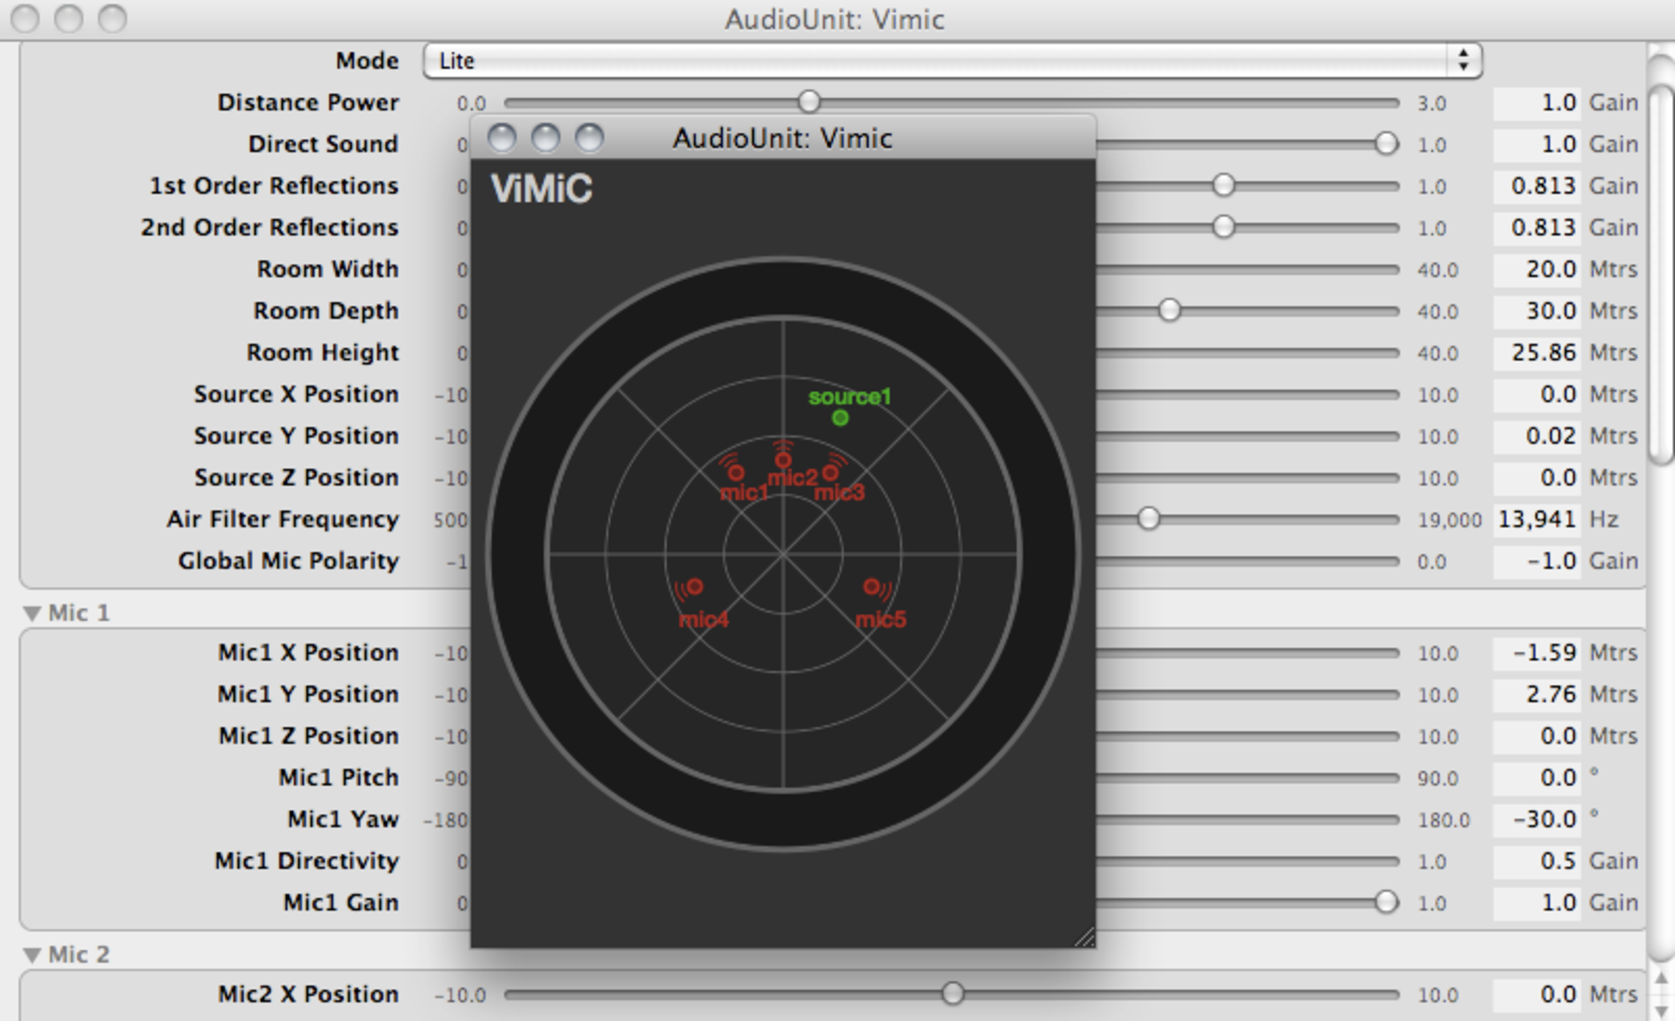
\includegraphics[width=0.9\columnwidth]{vimicAU.pdf}}}
\caption{ViMiC AU custom (front) and generic UI (back).}
\label{fig:vimic}
\end{figure}


\subsection{Ruby, IRB, Rails}

Ruby Language Bindings make the entirety of the DSP library accessible in the Ruby environment.  Together with Jamoma Multicore, Ruby's interactive shell (irb) can be use for live-coding by creating objects and manipulating the graph of those objects in real-time.  The following code shows a very simple irb session creating an instance of a lowpass filter, passing values one at a time through the filter.

% TODO: Nils, how do we make these lstlisting blocks use a small font size? (there are two of these blocks)
\begin{lstlisting}
    $ irb
    >> require 'TTRuby'
    JamomaFoundation -- Version 0.6
    JamomaDSP -- Version 0.6
    => true
    >> f = TTRuby.new("lowpass")
    => #<TTRuby:0x1011db170>
    >> f.calculate(1.0)
    => 0.25
    >> f.calculate(1.0)
    => 0.4375
\end{lstlisting}

Leveraging the popular Ruby on Rails web framework, Jamoma DSP classes are made available for a multitude of web applications.  The authors have begun employing one such Ruby on Rails application to graph related functions in real-time for comparison and algorithm analysis.


\subsection{Additional Environments}

Jamoma DSP includes further example projects wrapping classes for PureData and SuperCollider.

% (end)


%%%%%%%%%%%%%%%%%%%%%%%%%%%%%%%%%%%%%%%%%%%%%%%%%%%%%%%%%%%%%%%%%%%%%%%%%%%%%%%%%%%%%%%%%%%

\section{Discussion} % (fold)

% TODO: organize based on the terms in the abstract, and use this section to explain WHY these terms make this a good library.

% TODO: How do we explain this in 15 minutes so that it seems significant to someone new?
% _How_ do we go ahead to implement the fancy stuff that we required? Are there important design decisions involved that are worth presenting/discussing?
% What's Cool:
%   1. writing unit generators is clear and straight-forward (e.g. gain, delay, \ldots)  -- thanks in part to convention over configuration, DRY,...
%   2. combining unit generators is simple - example: combining simple units into compound (e.g. DC Blocker: see Section 'Examples')
%   3. wrapping for different environments is easy - this will be further improved in future using Jamoma Graphics

The class wrapper demonstrated in Section ? illustrates part of the power of the Jamoma Foundation for use as a \emph{rapid prototyping environment}.  It leverages all of the features of dynamic binding to make a class available to many different environments on many platforms with a minimal amount of coding and effort required.  The code base is further strengthened because this architecture provides a practical application of the DRY principle for representing concepts in a single authoritative location.  We can combine objects together in the environment of our choice: Max, Pd, a DAW (using plug-ins), or a web-browser using Ruby on Rails.  Then we can move the code from one environment to another easily, or port it back to C++ with minimal effort.

The Jamoma frameworks are all user-extensible through the creation of extension classes that are loaded and registered at runtime.  Future versions of Jamoma may provide additional means of defining extensions classes, including the ability to define extension classes in languages other than C++.

Introspection features of the Jamoma Foundation make it possible to query objects to automate the process of creating mappings and advanced control of the objects such as those cataloged in \cite{Pendharkar:2006}.  

A myriad of mundane, but critical, details for DSP classes are taken care of by the DSP framework.  This includes a 64-bit audio signal class that automatically adapts its channel configurations and vector-sizes based on input.  Multi-threaded environments seem to be the source of perpetual headaches, for developers.  Jamoma DSP provides a light-weight thread-protection where needed, but errs on the side of not getting in the way or causing performance problems.

% TODO: We have not addressed the next 3 in this section.  Do we need to? [tap]
%        - dynamically reconfigurable objects without recompiling code or DSP graphs
%            - FM example
%            - Live coding (irb?)

% CHANGED: We're short on space, so I mentioned DBAP as a one-liner in the Future Work secton [tap]
%[TL]    - DBAP interesting example of what kind of units Jamoma DSP can cater for
%        - split personality operating at audio and control rate
%            - two units tied together at runtime
%                - audio matrix
%                - coefficients for matrix calculated at control rate
%        - a biquad filter is really the same ....
%            - but if values at control rate can cause interpolation to new value, the ramp lib could get involved and we could choose what curve to use for interpolation (e.g. glissandi in the pitch domain)

% NOTE: Tim thinks the next paragraph should be the last of the Discussion section

The GNU LGPL license chosen for the Jamoma frameworks have enabled them to be used for open-source as well as commercial software development.  Electrotap's Tap.Tools\cite{web17} is a collection of externals for Max/MSP with an emphasis on audio effects processing.  They inherit multichannel audio support and 64-bit internal processing from the Jamoma DSP library.  Hipno\cite{Place:2005} is a set of audio effects plug-ins in the VST, RTAS and AudioUnit formats.  Hipno plug-ins were developed in Max/MSP with Tap.Tools and Jamoma DSP, using the now discontinued Cycling'74 Pluggo environment.  The cross-platform requirement detailed earlier has enabled Tap.tools, Hipno and Jamoma Modular to be developed for Mac OSX as well as Windows.  With the Jamoma Graphics library we wish to provide the structural framework for development of units with graphical user interfaces that can be wrapped as externals for environments such as Max, Pd and SuperCollider as well as being turned into plug-ins to replace now-obsolete infrastructure once provided by Pluggo.
    
% (end)


%%%%%%%%%%%%%%%%%%%%%%%%%%%%%%%%%%%%%%%%%%%%%%%%%%%%%%%%%%%%%%%%%%%%%%%%%%%%%%%%%%%%%%%%%%%

\section{Future Work} % (fold)

The class wrappers can be expanded to cover more environments, such as VST and SuperCollider, and CSound.

We need to do benchmarking, optimization, etc.  Work has already begun on SSE optimization, when available for the platform, in some classes.

% more units, support for common and well-established audio processing methods -  is it possible to borrow code from other projects where license permits it?
DSP Library expansion to include extensions for Spectral processing and Granular processing.  The EffectsLib can be expanded to cover standard effects including reverb, pitch-shifting, chorus, etc.  GeneratorLib can be expanded to cover a wider range of synthesis algorithms.  Of particular research interest are experimenting with applications of Non-linear filters - limiting or saturation inside the filter as xn is cast to xn-1 and yn to yn-1 (switching the feedback-filter on the fly).  Porting of DBAP to Jamoma DSP\cite{Lossius:2009}.

Initial work on a scheduler for the DSP library was begun in 2007.  Competing priorities have left it unfinished...  More interesting models for scheduling, such as the the model implemented in ChucK provide impetus for further research into new approaches to this topic.  We would like a sample-accurate scheduler like ChucK, but in a multi-threaded environment we will have a difficult time...

% CHANGED: Perhaps we should forget about the NodeLib for now, seems like too much of a tangent [tap]
% As a means of addressing parts of the system via OSC.  Somewhat like what Marsyas does.  An implementation of the ideas presented in\cite{Place:2008osc}.

In addition to the ongoing development of Jamoma Multicore, which implements an explicitly constructed graph of unit generators, a number of implicit graph-like processing structures such as those in Marsyas are of interest. %TODO: need the correct Marsyas citation for this!
In our current implementation it is possible to have a multichannel delay or filter class, for example.  However, the same coefficients are applied to each channel of the filter.  A paradigm in which each channel might possess distinct filter coefficients requires a grouping of filters such as an array that are treated as a unified entity in the graph.

% CHANGED: Web Browser Support (client-side) --  This is a distraction and not really relevant yet... [tap]

% (end)


%%%%%%%%%%%%%%%%%%%%%%%%%%%%%%%%%%%%%%%%%%%%%%%%%%%%%%%%%%%%%%%%%%%%%%%%%%%%%%%%%%%%%%%%%%%

\section{Summary} % (fold)

Jamoma Foundation and DSP provide a flexible, user-extendable, runtime environment for creating and using audio and digital signal processing objects.  Due to its advanced use of dynamic binding and message-passing paradigm, the building blocks can be reconfigured at runtime without requiring re-compilation, but with the unit generators themselves compiled as C++ and performing block-processing we retain the performance of a compiled language.

Perhaps more important, but more difficult to quantify, we believe we've created a context in which we code is `pleasant to work with'.  As stated by Lerch, ``A well-defined API can also speed up the development process, since the implementation can focus more on the algorithmic aspects and less on implementation issues like API design.'' \cite{Lerch:2005}

The power of this runtime is demonstrated through the ability to compile objects for Max, Pd, AudioUnits, VST, and Jamoma Multicore.

% (end)


%%%%%%%%%%%%%%%%%%%%%%%%%%%%%%%%%%%%%%%%%%%%%%%%%%%%%%%%%%%%%%%%%%%%%%%%%%%%%%%%%%%%%%%%%%%

\section{Acknowledgements} % (fold)

Dave Watson, Joshua Kit Clayton, Th\'eo Delahogue, Tristan Mathews

% (end)



%%%%%%%%% OLD STUFF FROM HERE ON

% To fully leverage the DSP library and Jamoma Foundation in a web-browser we need the ability to invoke the runtime on the client-side of the equation through a web browser plug-in similar to that done in the iARS Project\cite{Frauenberger:2003}.

% FM that can be repatching the FM unit in real time (different algorithms), like DX7 or Ableton Operator  -- (perhaps this could a part of the discussion section?) -- I would guess more here than in the multicore, as it's an example of dynamic binding between units





%%%%%%%%%%%%%%%%%%%%%%%%%%%%%%%%%%%%%%%%%%%%%%%%%%%%%%%%%%%%%%%%%%%%%%%%%%%%%%%%%%%%%%%%%%%

% TODO: Nils -- Why are the headings for the reference sections inconsistent with the rest of the template headings? [tap]

\bibliographystyle{IEEEtranS}
\bibliography{../../Shared/bibtex/Jamoma} % requires file template.bib
\renewcommand{\refname}{Web Resources}
\begin{thebibliography}{99}
	\footnotesize
\bibitem[A1]{web1}    \url{http://softwareengineering.vazexqi.com/files/pattern.html}
\bibitem[A2]{web2}    \url{http://www.extremeprogramming.org/rules/unittests.html}
\bibitem[A3]{web3}    \url{http://www.gnustep.org} 
\bibitem[A4]{web4}    \url{http://github.com/mhroth/ZenGarden}  
\bibitem[A5]{web5}    \url{http://rjdj.me} 
\bibitem[A6]{web6}    \url{http://en.wikipedia.org/wiki/OSI_model}
\bibitem[A7]{web7}    \url{http://github.com/tap/JamomaFoundation}     
\bibitem[A8]{web8}    \url{http://developer.apple.com/cocoa}    
\bibitem[A9]{web9} 	  \url{http://github.com/tap/JamomaDSP}
\bibitem[A10]{web10}  \url{http://github.com/tap/JamomaGraphics} 
\bibitem[A11]{web11}  \url{http://cairographics.org}
\bibitem[A12]{web12}  \url{http://github.com/tap/JamomaMulticore}
\bibitem[A13]{web13}  \url{http://github.com/tap/JamomaModular}
\bibitem[A14]{web14}  \url{http://github.com/tap/JamomaRuby}
\bibitem[A15]{web15}  \url{http://ruby-doc.org/docs/ProgrammingRuby/html/irb.html}
\bibitem[A16]{web16}  \url{http://rubyonrails.org}   
\bibitem[A17]{web17} \url{http://shop.electrotap.com/products/taptools}
\end{thebibliography} 
All quoted web resources were verified on \today.
\end{document}
